
%% bare_conf.tex
%% V1.3
%% 2007/01/11
%% by Michael Shell
%% See:
%% http://www.michaelshell.org/
%% for current contact information.
%%
%% This is a skeleton file demonstrating the use of IEEEtran.cls
%% (requires IEEEtran.cls version 1.7 or later) with an IEEE conference paper.
%%
%% Support sites:
%% http://www.michaelshell.org/tex/ieeetran/
%% http://www.ctan.org/tex-archive/macros/latex/contrib/IEEEtran/
%% and
%% http://www.ieee.org/

%%*************************************************************************
%% Legal Notice:
%% This code is offered as-is without any warranty either expressed or
%% implied; without even the implied warranty of MERCHANTABILITY or
%% FITNESS FOR A PARTICULAR PURPOSE! 
%% User assumes all risk.
%% In no event shall IEEE or any contributor to this code be liable for
%% any damages or losses, including, but not limited to, incidental,
%% consequential, or any other damages, resulting from the use or misuse
%% of any information contained here.
%%
%% All comments are the opinions of their respective authors and are not
%% necessarily endorsed by the IEEE.
%%
%% This work is distributed under the LaTeX Project Public License (LPPL)
%% ( http://www.latex-project.org/ ) version 1.3, and may be freely used,
%% distributed and modified. A copy of the LPPL, version 1.3, is included
%% in the base LaTeX documentation of all distributions of LaTeX released
%% 2003/12/01 or later.
%% Retain all contribution notices and credits.
%% ** Modified files should be clearly indicated as such, including  **
%% ** renaming them and changing author support contact information. **
%%
%% File list of work: IEEEtran.cls, IEEEtran_HOWTO.pdf, bare_adv.tex,
%%                    bare_conf.tex, bare_jrnl.tex, bare_jrnl_compsoc.tex
%%*************************************************************************

% *** Authors should verify (and, if needed, correct) their LaTeX system  ***
% *** with the testflow diagnostic prior to trusting their LaTeX platform ***
% *** with production work. IEEE's font choices can trigger bugs that do  ***
% *** not appear when using other class files.                            ***
% The testflow support page is at:
% http://www.michaelshell.org/tex/testflow/



% Note that the a4paper option is mainly intended so that authors in
% countries using A4 can easily print to A4 and see how their papers will
% look in print - the typesetting of the document will not typically be
% affected with changes in paper size (but the bottom and side margins will).
% Use the testflow package mentioned above to verify correct handling of
% both paper sizes by the user's LaTeX system.
%
% Also note that the "draftcls" or "draftclsnofoot", not "draft", option
% should be used if it is desired that the figures are to be displayed in
% draft mode.
%
\documentclass[10pt, conference, compsocconf]{IEEEtran}
% Add the compsocconf option for Computer Society conferences.
%
% If IEEEtran.cls has not been installed into the LaTeX system files,
% manually specify the path to it like:
% \documentclass[conference]{../sty/IEEEtran}





% Some very useful LaTeX packages include:
% (uncomment the ones you want to load)


% *** MISC UTILITY PACKAGES ***
%
%\usepackage{ifpdf}
% Heiko Oberdiek's ifpdf.sty is very useful if you need conditional
% compilation based on whether the output is pdf or dvi.
% usage:
% \ifpdf
%   % pdf code
% \else
%   % dvi code
% \fi
% The latest version of ifpdf.sty can be obtained from:
% http://www.ctan.org/tex-archive/macros/latex/contrib/oberdiek/
% Also, note that IEEEtran.cls V1.7 and later provides a builtin
% \ifCLASSINFOpdf conditional that works the same way.
% When switching from latex to pdflatex and vice-versa, the compiler may
% have to be run twice to clear warning/error messages.






% *** CITATION PACKAGES ***
%
%\usepackage{cite}
% cite.sty was written by Donald Arseneau
% V1.6 and later of IEEEtran pre-defines the format of the cite.sty package
% \cite{} output to follow that of IEEE. Loading the cite package will
% result in citation numbers being automatically sorted and properly
% "compressed/ranged". e.g., [1], [9], [2], [7], [5], [6] without using
% cite.sty will become [1], [2], [5]--[7], [9] using cite.sty. cite.sty's
% \cite will automatically add leading space, if needed. Use cite.sty's
% noadjust option (cite.sty V3.8 and later) if you want to turn this off.
% cite.sty is already installed on most LaTeX systems. Be sure and use
% version 4.0 (2003-05-27) and later if using hyperref.sty. cite.sty does
% not currently provide for hyperlinked citations.
% The latest version can be obtained at:
% http://www.ctan.org/tex-archive/macros/latex/contrib/cite/
% The documentation is contained in the cite.sty file itself.






% *** GRAPHICS RELATED PACKAGES ***
%
\ifCLASSINFOpdf
  % \usepackage[pdftex]{graphicx}
  % declare the path(s) where your graphic files are
  % \graphicspath{{../pdf/}{../jpeg/}}
  % and their extensions so you won't have to specify these with
  % every instance of \includegraphics
  % \DeclareGraphicsExtensions{.pdf,.jpeg,.png}
\else
  % or other class option (dvipsone, dvipdf, if not using dvips). graphicx
  % will default to the driver specified in the system graphics.cfg if no
  % driver is specified.
  % \usepackage[dvips]{graphicx}
  % declare the path(s) where your graphic files are
  % \graphicspath{{../eps/}}
  % and their extensions so you won't have to specify these with
  % every instance of \includegraphics
  % \DeclareGraphicsExtensions{.eps}
\fi
% graphicx was written by David Carlisle and Sebastian Rahtz. It is
% required if you want graphics, photos, etc. graphicx.sty is already
% installed on most LaTeX systems. The latest version and documentation can
% be obtained at: 
% http://www.ctan.org/tex-archive/macros/latex/required/graphics/
% Another good source of documentation is "Using Imported Graphics in
% LaTeX2e" by Keith Reckdahl which can be found as epslatex.ps or
% epslatex.pdf at: http://www.ctan.org/tex-archive/info/
%
% latex, and pdflatex in dvi mode, support graphics in encapsulated
% postscript (.eps) format. pdflatex in pdf mode supports graphics
% in .pdf, .jpeg, .png and .mps (metapost) formats. Users should ensure
% that all non-photo figures use a vector format (.eps, .pdf, .mps) and
% not a bitmapped formats (.jpeg, .png). IEEE frowns on bitmapped formats
% which can result in "jaggedy"/blurry rendering of lines and letters as
% well as large increases in file sizes.
%
% You can find documentation about the pdfTeX application at:
% http://www.tug.org/applications/pdftex





% *** MATH PACKAGES ***
%
%\usepackage[cmex10]{amsmath}
% A popular package from the American Mathematical Society that provides
% many useful and powerful commands for dealing with mathematics. If using
% it, be sure to load this package with the cmex10 option to ensure that
% only type 1 fonts will utilized at all point sizes. Without this option,
% it is possible that some math symbols, particularly those within
% footnotes, will be rendered in bitmap form which will result in a
% document that can not be IEEE Xplore compliant!
%
% Also, note that the amsmath package sets \interdisplaylinepenalty to 10000
% thus preventing page breaks from occurring within multiline equations. Use:
%\interdisplaylinepenalty=2500
% after loading amsmath to restore such page breaks as IEEEtran.cls normally
% does. amsmath.sty is already installed on most LaTeX systems. The latest
% version and documentation can be obtained at:
% http://www.ctan.org/tex-archive/macros/latex/required/amslatex/math/





% *** SPECIALIZED LIST PACKAGES ***
%
%\usepackage{algorithmic}
% algorithmic.sty was written by Peter Williams and Rogerio Brito.
% This package provides an algorithmic environment fo describing algorithms.
% You can use the algorithmic environment in-text or within a figure
% environment to provide for a floating algorithm. Do NOT use the algorithm
% floating environment provided by algorithm.sty (by the same authors) or
% algorithm2e.sty (by Christophe Fiorio) as IEEE does not use dedicated
% algorithm float types and packages that provide these will not provide
% correct IEEE style captions. The latest version and documentation of
% algorithmic.sty can be obtained at:
% http://www.ctan.org/tex-archive/macros/latex/contrib/algorithms/
% There is also a support site at:
% http://algorithms.berlios.de/index.html
% Also of interest may be the (relatively newer and more customizable)
% algorithmicx.sty package by Szasz Janos:
% http://www.ctan.org/tex-archive/macros/latex/contrib/algorithmicx/




% *** ALIGNMENT PACKAGES ***
%
%\usepackage{array}
% Frank Mittelbach's and David Carlisle's array.sty patches and improves
% the standard LaTeX2e array and tabular environments to provide better
% appearance and additional user controls. As the default LaTeX2e table
% generation code is lacking to the point of almost being broken with
% respect to the quality of the end results, all users are strongly
% advised to use an enhanced (at the very least that provided by array.sty)
% set of table tools. array.sty is already installed on most systems. The
% latest version and documentation can be obtained at:
% http://www.ctan.org/tex-archive/macros/latex/required/tools/


%\usepackage{mdwmath}
%\usepackage{mdwtab}
% Also highly recommended is Mark Wooding's extremely powerful MDW tools,
% especially mdwmath.sty and mdwtab.sty which are used to format equations
% and tables, respectively. The MDWtools set is already installed on most
% LaTeX systems. The lastest version and documentation is available at:
% http://www.ctan.org/tex-archive/macros/latex/contrib/mdwtools/


% IEEEtran contains the IEEEeqnarray family of commands that can be used to
% generate multiline equations as well as matrices, tables, etc., of high
% quality.


%\usepackage{eqparbox}
% Also of notable interest is Scott Pakin's eqparbox package for creating
% (automatically sized) equal width boxes - aka "natural width parboxes".
% Available at:
% http://www.ctan.org/tex-archive/macros/latex/contrib/eqparbox/





% *** SUBFIGURE PACKAGES ***
%\usepackage[tight,footnotesize]{subfigure}
% subfigure.sty was written by Steven Douglas Cochran. This package makes it
% easy to put subfigures in your figures. e.g., "Figure 1a and 1b". For IEEE
% work, it is a good idea to load it with the tight package option to reduce
% the amount of white space around the subfigures. subfigure.sty is already
% installed on most LaTeX systems. The latest version and documentation can
% be obtained at:
% http://www.ctan.org/tex-archive/obsolete/macros/latex/contrib/subfigure/
% subfigure.sty has been superceeded by subfig.sty.



%\usepackage[caption=false]{caption}
%\usepackage[font=footnotesize]{subfig}
% subfig.sty, also written by Steven Douglas Cochran, is the modern
% replacement for subfigure.sty. However, subfig.sty requires and
% automatically loads Axel Sommerfeldt's caption.sty which will override
% IEEEtran.cls handling of captions and this will result in nonIEEE style
% figure/table captions. To prevent this problem, be sure and preload
% caption.sty with its "caption=false" package option. This is will preserve
% IEEEtran.cls handing of captions. Version 1.3 (2005/06/28) and later 
% (recommended due to many improvements over 1.2) of subfig.sty supports
% the caption=false option directly:
%\usepackage[caption=false,font=footnotesize]{subfig}
%
% The latest version and documentation can be obtained at:
% http://www.ctan.org/tex-archive/macros/latex/contrib/subfig/
% The latest version and documentation of caption.sty can be obtained at:
% http://www.ctan.org/tex-archive/macros/latex/contrib/caption/




% *** FLOAT PACKAGES ***
%
%\usepackage{fixltx2e}
% fixltx2e, the successor to the earlier fix2col.sty, was written by
% Frank Mittelbach and David Carlisle. This package corrects a few problems
% in the LaTeX2e kernel, the most notable of which is that in current
% LaTeX2e releases, the ordering of single and double column floats is not
% guaranteed to be preserved. Thus, an unpatched LaTeX2e can allow a
% single column figure to be placed prior to an earlier double column
% figure. The latest version and documentation can be found at:
% http://www.ctan.org/tex-archive/macros/latex/base/



%\usepackage{stfloats}
% stfloats.sty was written by Sigitas Tolusis. This package gives LaTeX2e
% the ability to do double column floats at the bottom of the page as well
% as the top. (e.g., "\begin{figure*}[!b]" is not normally possible in
% LaTeX2e). It also provides a command:
%\fnbelowfloat
% to enable the placement of footnotes below bottom floats (the standard
% LaTeX2e kernel puts them above bottom floats). This is an invasive package
% which rewrites many portions of the LaTeX2e float routines. It may not work
% with other packages that modify the LaTeX2e float routines. The latest
% version and documentation can be obtained at:
% http://www.ctan.org/tex-archive/macros/latex/contrib/sttools/
% Documentation is contained in the stfloats.sty comments as well as in the
% presfull.pdf file. Do not use the stfloats baselinefloat ability as IEEE
% does not allow \baselineskip to stretch. Authors submitting work to the
% IEEE should note that IEEE rarely uses double column equations and
% that authors should try to avoid such use. Do not be tempted to use the
% cuted.sty or midfloat.sty packages (also by Sigitas Tolusis) as IEEE does
% not format its papers in such ways.





% *** PDF, URL AND HYPERLINK PACKAGES ***
%
%\usepackage{url}
% url.sty was written by Donald Arseneau. It provides better support for
% handling and breaking URLs. url.sty is already installed on most LaTeX
% systems. The latest version can be obtained at:
% http://www.ctan.org/tex-archive/macros/latex/contrib/misc/
% Read the url.sty source comments for usage information. Basically,
% \url{my_url_here}.

\usepackage{graphicx}



% *** Do not adjust lengths that control margins, column widths, etc. ***
% *** Do not use packages that alter fonts (such as pslatex).         ***
% There should be no need to do such things with IEEEtran.cls V1.6 and later.
% (Unless specifically asked to do so by the journal or conference you plan
% to submit to, of course. )

\newtheorem{theorem}{Theorem}
% correct bad hyphenation here
\hyphenation{op-tical net-works semi-conduc-tor}


\begin{document}
%
% paper title
% can use linebreaks \\ within to get better formatting as desired
\title{M4: A Visualization-Oriented Time Series Data Aggregation
}


% author names and affiliations
% use a multiple column layout for up to two different
% affiliations

\author{\IEEEauthorblockN{Uwe Jugel, Zbigniew Jerzak,}
\IEEEauthorblockA{ Gregor Hackenbroich\\
SAP AG\\
Chemnitzer Str. 48, 01187 Dresden, Germany\\}
\and
\IEEEauthorblockN{Volker Markl}
\IEEEauthorblockA{Technische Universitat Berlin\\
Straße des 17. Juni 135\\
10623 Berlin, Germany\\
volker.markl@tu-berlin.de}
}

% conference papers do not typically use \thanks and this command
% is locked out in conference mode. If really needed, such as for
% the acknowledgment of grants, issue a \IEEEoverridecommandlockouts
% after \documentclass

% for over three affiliations, or if they all won't fit within the width
% of the page, use this alternative format:
% 
%\author{\IEEEauthorblockN{Michael Shell\IEEEauthorrefmark{1},
%Homer Simpson\IEEEauthorrefmark{2},
%James Kirk\IEEEauthorrefmark{3}, 
%Montgomery Scott\IEEEauthorrefmark{3} and
%Eldon Tyrell\IEEEauthorrefmark{4}}
%\IEEEauthorblockA{\IEEEauthorrefmark{1}School of Electrical and Computer Engineering\\
%Georgia Institute of Technology,
%Atlanta, Georgia 30332--0250\\ Email: see http://www.michaelshell.org/contact.html}
%\IEEEauthorblockA{\IEEEauthorrefmark{2}Twentieth Century Fox, Springfield, USA\\
%Email: homer@thesimpsons.com}
%\IEEEauthorblockA{\IEEEauthorrefmark{3}Starfleet Academy, San Francisco, California 96678-2391\\
%Telephone: (800) 555--1212, Fax: (888) 555--1212}
%\IEEEauthorblockA{\IEEEauthorrefmark{4}Tyrell Inc., 123 Replicant Street, Los Angeles, California 90210--4321}}




% use for special paper notices
%\IEEEspecialpapernotice{(Invited Paper)}




% make the title area
\maketitle


%\begin{abstract}
%The abstract goes here. DO NOT USE SPECIAL CHARACTERS, SYMBOLS, OR MATH IN YOUR TITLE OR ABSTRACT.

%\end{abstract}

%\begin{IEEEkeywords}
%component; formatting; style; styling;

%\end{IEEEkeywords}


% For peer review papers, you can put extra information on the cover
% page as needed:
% \ifCLASSOPTIONpeerreview
% \begin{center} \bfseries EDICS Category: 3-BBND \end{center}
% \fi
%
% For peerreview papers, this IEEEtran command inserts a page break and
% creates the second title. It will be ignored for other modes.
\IEEEpeerreviewmaketitle



\section{Introduction} \label{intro}
Visualization of large scale time series data is a crucial need of modern exploratory
bigdata analysis \cite{fu2011review}. But the huge size of the data is a barrier to visualization \cite{labrinidis2012challenges,fan2014challenges,chen2014data}. 
To address this challenge of bigdata different data reduction and sampling strategies are used to overcome the barrier \cite{cormode2014sampling,wu2014data}. But for preserving the 
semantics of trend line of time series data these sampling strategies show huge 
limitations \cite{jugel2014m4}. 

In this review paper we present a review of the paper \cite{jugel2014m4} which address this issue of preserving the semantic of time series data and present some related works in the line.  The paper appeared in the Proceedings of the VLDB Endowment, 2014. 

The authors present M4, an aggregation based time series data reduction strategy that guarantees error free visualization of time series data as line chart as well as higher rate of data reduction. The approach is generic to any visualization system as long as the visualization systems uses RDBMS as data source.  
\section{Controbutions of the paper}
The authors of the paper rewrite visualization queries $Q$ using data reduction operator 
$M_R$ such that the visualization of the original data from query $Q$ and the visualization 
from the query $Q_R = M_R(Q)$ are similar and error free. 
\begin{figure}[h]
	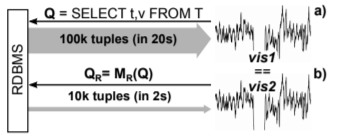
\includegraphics[width=0.5\textwidth]{qr}
	\caption{Time series visualization: a) based on original data; b) Using data reduction operator;}   
	\label{fig:1}
\end{figure}
As shown in Figure \ref{fig:1} $Q_R$ produced the same visualization as $Q$ with almost 10 times less tuples and 10 times reduced time. 

\section{Query Rewriting}
TODO
\section{Time Series Visualization}
TODO
\section{Data Reduction Operators}
TODO
\section{Time Series Data Reduction}


\section{Evaluation}
The authors use three different real life time series data and evaluate their results with some existing state of the art data reduction approaches.
The authors use the following datasets:
\begin{enumerate}
	\item the price of a single
	share on the Frankfurt stock exchange over 6 weeks (700k
	tuples)
	\item 71 minutes from a speed sensor of a soccer ball
	\cite{mutschler2013debs}(ball number 8, 7M rows)
	\item one week of sensor data
	from an electrical power sensor of a semiconductor manufacturing
	machine \cite{jerzak2012debs}(sensor MF03, 55M rows)
\end{enumerate}

The approaches compared are following:
1) a baseline query that selects
all tuples to be visualized, 2) a PAA-query that computes
up to 4·w average tuples, 3) a two-dimensional rounding
query that selects up to w.h rounded tuples, 4) a strati-
fied random sampling query that selects 4·w random tuples,
5) a systematic sampling query that selects 4·w first tuples,
6) a MinMax query that selects the two min and max tuples
from 2 · w groups, and finally 7)  M4 query selecting
all four extrema from w groups.

\subsection{Query performance}
\begin{figure*}
	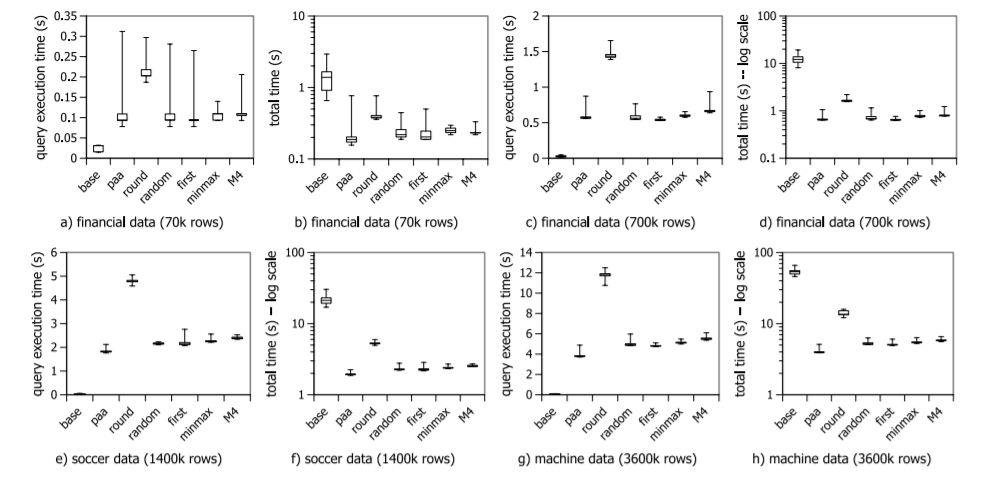
\includegraphics[width=\textwidth]{qp}
	\caption{Query performance: (a,b,c,d) financial data, (e,f) soccer data, (g,h) machine data}
	\label{qper}
\end{figure*}

\begin{figure*}
	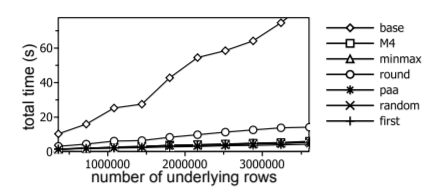
\includegraphics[width=0.5\textwidth]{pv}
	\caption{Performance of different queries with varying row counts}
	\label{vr}
\end{figure*}
\begin{figure*}
	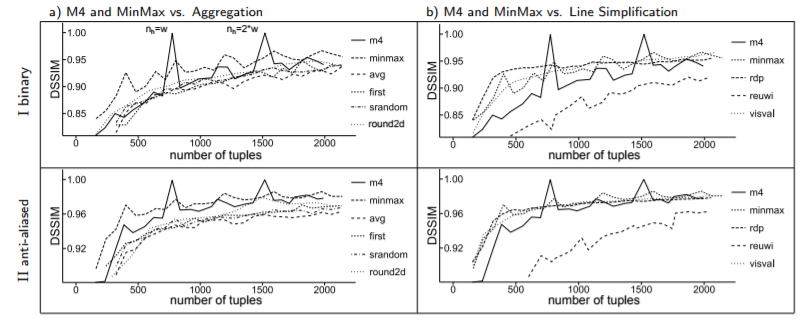
\includegraphics[width=\textwidth]{dsim}
	\caption{: Data efficiency of evaluated techniques, showing DSSIM over data volume}
	\label{dsim}
\end{figure*}

The query performance of different approaches in terms of execution time of the queries is shown in Figure \ref{qper}. It shows that aggregation based approaches perform better compared to baseline approaches. Figure \ref{vr} shows exemplary results of performance  for varying row counts on soccer data. The aggregation based queries perform much than baseline queries as the size of rows increase. 

\subsection{Visualization quality and Data Efficiency}
Authors in \cite{wang2004image} have shown that for visualization quality $MSE$ (Mean Square Error) doesn't perform well and they proposed $SSIM$ (Structural
Similarity Index) for the measurement of image quality. The SSIM yields a similarity
value between 1 and −1. The authors use $DSSIM$, the normalized distance between two visualizations for measuring the visualization quality. The formula is given below:
\begin{equation}
DSSIM(V_1, V_2) = \frac{1 - SSIM}{2}
\end{equation}

In Figure \ref{dsim}, the authors plotted the measured, resulting visualization
quality (DSSIM) over the resulting number of tuples of each
different groupings $n_h = 1$ to $n_h = 2.5·w$ of an applied data
reduction technique. The lower the number of
tuples and the higher the DSSIM, the more data efficient is
the corresponding technique for the purpose of line visualization.
The Figures \ref{dsim}aI and \ref{dsim}bI depict these measures for
binary line visualizations and the Figures \ref{dsim}aII and \ref{dsim}bII
for anti-aliased line visualizations. We now observe the following
results.

\section{Prior Works}
In this section, various prior works in the field of visualization systems has been discussed.

\begin{enumerate}
	\item Visualization Systems
\end{enumerate}
Current Visualization systems are categorized into three categories 1) The ones which do not used data reduction 2) The ones that compute and send images instead to data visualization 3) The ones which rely upon data reduction outside of the database.

These three approaches have been compared with the authors’ proposed solution.\newline


\textit{Visual Analytic Tools – }
Tools such as Tableu, SAP Lumira, QlikView, and Datawatch fall into first category, i.e. they do not apply any data reduction related to visualization, even though they contain the most recent and advanced data engines. None of these tools can efficiently process and visualize data having more than 1 million rows. There is a great opportunity to implement the proposed solution in this paper along with these softwares. \newline


\textit{Client Server Systems –  }
Online data visualization websites like Yahoo Finance, or Google Finance come under second category. They reduce data volumes by generating images instead of actual data visualization. They are dependent upon client systems to interact with these images to explore data. These systems rely on additional data reduction or image generation components between the data-engine and the client. Transferring large query results to external image generation or data reduction components will negatively impact the system performance as data transfer is one of the costliest operations. \newline



\textit{Data-Centric Systems -}
The third category of systems consist of rich-client visualization systems which are also described in the section above. Authors’ proposed system can prevent the costly data transfer by running the expensive data reduction operations directly inside the data engine. The system modifies the original query by adding in some data reduction operations and then runs the new query. The data engine can then execute this new query, thus performing the additional data reduction task without the need of data transfer.\newline



\begin{enumerate}
	\item Data Reduction
\end{enumerate}

In this section, the author talks about the pre-existing data reduction methods and how they are related to visualization.\newline

\textit{Quantization - }
Most visualization systems reduce the continuos time series data into discrete values, by generating images or rounding of the decimal integers. This does not allow correct reproduction of original data. \newline

\textit{Time-Series Representation -}
The goal of existing works on time-series representation is to obtain a much smaller representation of the complete time-series. This is often achieved by dividing the time series into various intervals and calculating the average of those intervals. This result is the approximation of original time series. The authors in addition to these methods have focused on relational operators and incorporated the semantics of visualizations. \newline

In addition to the above pre-existing methods there are some other methods which focus on \textit{offline Aggregation and synopsis, Data Compression, Content Adaption, and various statistical approaches}. In offline aggregation technique, some aggregation methods like sum, avg, count of data are implemented which approximately represent the data, but they still are subjected to approximation errors. Data Compression is applied on application level data till now. Authors’techniques can also be applied to transport level data such as data packet compression. There are different data reduction techniques for different kind of contents. The proposed solution in this paper can be applied to any kind of content like videos, images, or text in web based systems.
\newline


\begin{enumerate}
	\item Visualization-Driven Data Reduction 
\end{enumerate}

Burtini et al. [12] has described the usage of visualization parameters for data reduction. Howeverm they describe a client-server system as described earlier in category 3, i.e., they apply data reduction outside of the database. In the proposed solution, all the data processing including the data reduction is processed by the means of modified queries. Also, previous works use aggregation techniques for data reduction thus losing the important details in the vertical extrema and do not discuss the semantics of rasterized line visualizations as covered in this paper. 

\section{Our Proposal}
Though the M4 aggregation provides an error free visualization it has the following limitations:
\begin{enumerate}
	\item It doesn't work with other data sources besides RDBMS
	\item It doesn't provide solution to map-reduce based big data frame works like Hadoop, spark etc.
	\item and it doesn't handle the data file system like CSV, JSON and most visualization systems take data directly from these file systems \cite{bostock2011d3}.
	\item It also doesn't provide solution for streaming data visualizations. But visualization of streaming time series data with appropriate reduction in data size is a crucial need of moder exploratory data analysis etc.
\end{enumerate}
We propose some improvements and future works that can be done on top of this works.
\begin{itemize}
	\item To cover the modern NoSQL databases like MongoDB and cluster based daat sources like Hadoop and spark we need to modify the M4 aggregation strategies and adapt those to MongoDB NoSQL queries and Hadoop Map-reduce queries. It can be easily shown that the M4 query can be adapted to these platforms after slight modifications. For example if we write map-reduce queries using Apache Hive \cite{thusoo2009hive,barbierato2013modeling} that comes with Hadoop stack the same SQL queries used by M4 can be used.
\end{itemize}

% An example of a floating figure using the graphicx package.
% Note that \label must occur AFTER (or within) \caption.
% For figures, \caption should occur after the \includegraphics.
% Note that IEEEtran v1.7 and later has special internal code that
% is designed to preserve the operation of \label within \caption
% even when the captionsoff option is in effect. However, because
% of issues like this, it may be the safest practice to put all your
% \label just after \caption rather than within \caption{}.
%
% Reminder: the "draftcls" or "draftclsnofoot", not "draft", class
% option should be used if it is desired that the figures are to be
% displayed while in draft mode.
%
%\begin{figure}[!t]
%\centering
%\includegraphics[width=2.5in]{myfigure}
% where an .eps filename suffix will be assumed under latex, 
% and a .pdf suffix will be assumed for pdflatex; or what has been declared
% via \DeclareGraphicsExtensions.
%\caption{Simulation Results}
%\label{fig_sim}
%\end{figure}

% Note that IEEE typically puts floats only at the top, even when this
% results in a large percentage of a column being occupied by floats.


% An example of a double column floating figure using two subfigures.
% (The subfig.sty package must be loaded for this to work.)
% The subfigure \label commands are set within each subfloat command, the
% \label for the overall figure must come after \caption.
% \hfil must be used as a separator to get equal spacing.
% The subfigure.sty package works much the same way, except \subfigure is
% used instead of \subfloat.
%
%\begin{figure*}[!t]
%\centerline{\subfloat[Case I]\includegraphics[width=2.5in]{subfigcase1}%
%\label{fig_first_case}}
%\hfil
%\subfloat[Case II]{\includegraphics[width=2.5in]{subfigcase2}%
%\label{fig_second_case}}}
%\caption{Simulation results}
%\label{fig_sim}
%\end{figure*}
%
% Note that often IEEE papers with subfigures do not employ subfigure
% captions (using the optional argument to \subfloat), but instead will
% reference/describe all of them (a), (b), etc., within the main caption.


% An example of a floating table. Note that, for IEEE style tables, the 
% \caption command should come BEFORE the table. Table text will default to
% \footnotesize as IEEE normally uses this smaller font for tables.
% The \label must come after \caption as always.
%
%\begin{table}[!t]
%% increase table row spacing, adjust to taste
%\renewcommand{\arraystretch}{1.3}
% if using array.sty, it might be a good idea to tweak the value of
% \extrarowheight as needed to properly center the text within the cells
%\caption{An Example of a Table}
%\label{table_example}
%\centering
%% Some packages, such as MDW tools, offer better commands for making tables
%% than the plain LaTeX2e tabular which is used here.
%\begin{tabular}{|c||c|}
%\hline
%One & Two\\
%\hline
%Three & Four\\
%\hline
%\end{tabular}
%\end{table}


% Note that IEEE does not put floats in the very first column - or typically
% anywhere on the first page for that matter. Also, in-text middle ("here")
% positioning is not used. Most IEEE journals/conferences use top floats
% exclusively. Note that, LaTeX2e, unlike IEEE journals/conferences, places
% footnotes above bottom floats. This can be corrected via the \fnbelowfloat
% command of the stfloats package.



\section{Conclusion}
The conclusion goes here. this is more of the conclusion

% conference papers do not normally have an appendix


% use section* for acknowledgement


% trigger a \newpage just before the given reference
% number - used to balance the columns on the last page
% adjust value as needed - may need to be readjusted if
% the document is modified later
%\IEEEtriggeratref{8}
% The "triggered" command can be changed if desired:
%\IEEEtriggercmd{\enlargethispage{-5in}}

% references section

% can use a bibliography generated by BibTeX as a .bbl file
% BibTeX documentation can be easily obtained at:
% http://www.ctan.org/tex-archive/biblio/bibtex/contrib/doc/
% The IEEEtran BibTeX style support page is at:
% http://www.michaelshell.org/tex/ieeetran/bibtex/
\bibliographystyle{IEEEtran}
% argument is your BibTeX string definitions and bibliography database(s)
\bibliography{IEEEabrv}
%
% <OR> manually copy in the resultant .bbl file
% set second argument of \begin to the number of references
% (used to reserve space for the reference number labels box)
%\begin{thebibliography}{1}

%\bibitem{IEEEhowto:kopka}
%H.~Kopka and P.~W. Daly, \emph{A Guide to \LaTeX}, 3rd~ed.\hskip 1em plus
%  0.5em minus 0.4em\relax Harlow, England: Addison-Wesley, 1999.

%\end{thebibliography}




% that's all folks
\end{document}


